\begin{figure}[t]
\centering
\definecolor{cVer}{HTML}{0072B2}   % verified (computer-algebra) pairs
\definecolor{cRec}{HTML}{D55E00}   % recipe-family prompts D1-D3
\definecolor{cD4}{HTML}{E69F00}    % D4 restatements (unrelated prompt)
\definecolor{cBT}{HTML}{009E73}    % back-translated positives
\definecolor{cMELD}{HTML}{999999}  % MELD-recipe arm
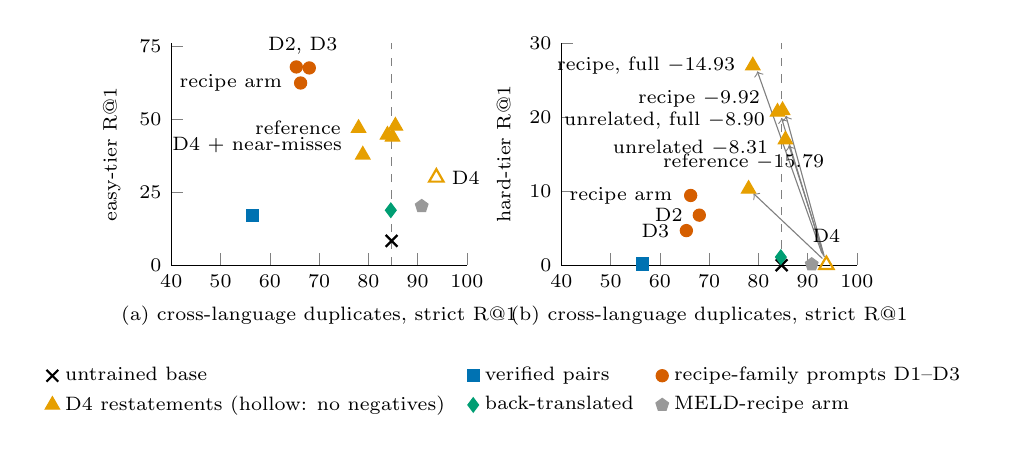
\begin{tikzpicture}
\begin{axis}[
  name=a,
  width=0.44\linewidth, height=4.4cm,
  xmin=40, xmax=100, ymin=0, ymax=76,
  xtick={40,50,60,70,80,90,100}, ytick={0,25,50,75},
  xlabel={(a) cross-language duplicates, strict R@1}, ylabel={easy-tier R@1},
  label style={font=\scriptsize}, tick label style={font=\scriptsize},
  axis y line*=left, axis x line*=bottom, clip=false,
]
\addplot[gray, dashed, forget plot] coordinates {(84.73,0) (84.73,76)};
\addplot[forget plot, only marks, mark=x, mark size=3pt, thick, black] coordinates {(84.73,8.32)};
\addplot[forget plot, only marks, mark=square*, mark size=2.2pt, cVer] coordinates {(56.52,17.05)};
\addplot[forget plot, only marks, mark=*, mark size=2.2pt, cRec] coordinates {(66.26,62.38) (68.02,67.54) (65.39,67.88)};
\addplot[forget plot, only marks, mark=triangle, mark size=3pt, thick, cD4] coordinates {(93.81,30.03)};
\addplot[forget plot, only marks, mark=triangle*, mark size=3pt, cD4] coordinates {(78.02,46.91) (83.89,44.59) (78.88,37.79) (85.50,47.69) (84.91,43.93)};
\addplot[forget plot, only marks, mark=diamond*, mark size=2.6pt, cBT] coordinates {(84.57,18.81)};
\addplot[forget plot, only marks, mark=pentagon*, mark size=2.4pt, cMELD] coordinates {(90.84,20.23)};
\node[font=\scriptsize, anchor=east] at (axis cs:64.5,62.38) {recipe arm};
\node[font=\scriptsize, anchor=south] at (axis cs:66.7,69.0) {D2, D3};
\node[font=\scriptsize, anchor=west] at (axis cs:95.0,30.03) {D4};
\node[font=\scriptsize, anchor=east] at (axis cs:76.4,46.91) {reference};
\node[font=\scriptsize, anchor=east] at (axis cs:76.6,41.2) {D4 + near-misses};
\end{axis}
\begin{axis}[
  name=b, at={(a.south east)}, anchor=south west, xshift=1.2cm,
  width=0.44\linewidth, height=4.4cm,
  xmin=40, xmax=100, ymin=0, ymax=30,
  xtick={40,50,60,70,80,90,100}, ytick={0,10,20,30},
  xlabel={(b) cross-language duplicates, strict R@1}, ylabel={hard-tier R@1},
  label style={font=\scriptsize}, tick label style={font=\scriptsize},
  axis y line*=left, axis x line*=bottom, clip=false,
  legend to name=invlegend, legend columns=3,
  legend style={font=\scriptsize, draw=none, /tikz/every even column/.append style={column sep=6pt}}, legend cell align=left,
]
\addplot[gray, dashed, forget plot] coordinates {(84.73,0) (84.73,30)};
\addplot[only marks, mark=x, mark size=3pt, thick, black] coordinates {(84.73,0.00)};
\addlegendentry{untrained base}
\addplot[only marks, mark=square*, mark size=2.2pt, cVer] coordinates {(56.52,0.16)};
\addlegendentry{verified pairs}
\addplot[only marks, mark=*, mark size=2.2pt, cRec] coordinates {(66.26,9.42) (68.02,6.76) (65.39,4.67)};
\addlegendentry{recipe-family prompts D1--D3}
\addplot[only marks, mark=triangle*, mark size=3pt, cD4] coordinates {(78.02,10.30) (83.89,20.71) (78.88,26.97) (85.50,16.96) (84.91,20.93)};
\addlegendentry{D4 restatements (hollow: no negatives)}
\addplot[forget plot, only marks, mark=triangle, mark size=3pt, thick, cD4] coordinates {(93.81,0.04)};
\addplot[only marks, mark=diamond*, mark size=2.6pt, cBT] coordinates {(84.57,1.09)};
\addlegendentry{back-translated}
\addplot[only marks, mark=pentagon*, mark size=2.4pt, cMELD] coordinates {(90.84,0.11)};
\addlegendentry{MELD-recipe arm}
\draw[->, thin, gray] (axis cs:93.0,0.9) -- (axis cs:79.0,9.7);
\draw[->, thin, gray] (axis cs:93.2,1.3) -- (axis cs:84.7,19.9);
\draw[->, thin, gray] (axis cs:92.9,1.6) -- (axis cs:79.8,26.2);
\draw[->, thin, gray] (axis cs:93.4,1.1) -- (axis cs:86.2,16.2);
\draw[->, thin, gray] (axis cs:93.3,1.4) -- (axis cs:85.6,20.2);
\node[font=\scriptsize, anchor=east] at (axis cs:64.5,9.42) {recipe arm};
\node[font=\scriptsize, anchor=east] at (axis cs:66.6,6.76) {D2};
\node[font=\scriptsize, anchor=east] at (axis cs:63.9,4.67) {D3};
\node[font=\scriptsize, anchor=south] at (axis cs:93.81,1.8) {D4};
\node[font=\scriptsize, anchor=south] at (axis cs:77.0,11.6) {reference $-15.79$};
\node[font=\scriptsize, anchor=east] at (axis cs:77.3,26.97) {recipe, full $-14.93$};
\node[font=\scriptsize, anchor=east] at (axis cs:82.3,22.5) {recipe $-9.92$};
\node[font=\scriptsize, anchor=east] at (axis cs:83.3,19.5) {unrelated, full $-8.90$};
\node[font=\scriptsize, anchor=east] at (axis cs:84.0,15.9) {unrelated $-8.31$};
\end{axis}
\node[anchor=north, yshift=-4pt] at (current bounding box.south) {\pgfplotslegendfromname{invlegend}};
\end{tikzpicture}
\caption{Benchmark score against real retrieval kept after training, one point per trained model. Horizontal axis: strict R@1 on cross-language duplicates; the dashed line and $\times$ mark the untrained base, so points left of it lost real retrieval by being trained. Colour gives the positives (legend); hollow means no negatives. (a)~Easy tier: every model trained on LLM rewrites scores above the verified arm. (b)~Hard tier: only deep LLM rewrites with negatives leave the floor. Arrows run from D4 alone to D4 with negatives attached; each label names the negatives (verified ones give the reference; ``recipe'' and ``unrelated'' are LLM near-misses from the recipe's prompt and from an unrelated one, at the reference's count or at the recipe arm's full volume) and the cross-language points lost. All models: Figure~\ref{fig:inversion-full}.}
\label{fig:inversion}
\end{figure}